\section{Marco teórico}

En esta sección se desarrollarán los principios teóricos que permiten el funcionamiento de las lanzaderas electromagnéticas. Para entender estos principios, es esencial comprender los fundamentos del electromagnetismo, el concepto de bobina y su relación con la generación de campos magnéticos.

El electromagnetismo es una rama fundamental de la física que estudia las interacciones entre los campos eléctricos y magnéticos. Su desarrollo ha sido crucial para el avance de la tecnología, desde la generación y transmisión de electricidad hasta las comunicaciones inalámbricas. Aunque la raza humana conoce los fenómenos eléctricos y magnéticos desde la historia antigua, estos no fueron estudiados hasta el siglo XVII, y se consideraban fenómenos independientes hasta que Hans Christian Ørsted descubrió en 1820 que una corriente eléctrica puede generar un campo magnético. Mientras el físico danés preparaba los equipos para dar una conferencia en la Universidad de Copenhague, observó que la aguja de una brújula cercana se desviaba cuando la corriente fluía a través de un alambre conductor. Este accidental descubrimiento le llevó a publicar el artículo CIRCA EFFECTUM CONFLICTUS ELECTRICI IN ACUM MAGNETICAM, en el que se describieron los fenómenos electromagnéticos por primera vez, aunque de manera cualitativa. En la siguiente década, Ampère y Faraday describirían matemáticamente el descubrimiento de Ørsted, dando lugar al electromagnetismo como lo conocemos hoy en día. \citep{oersted2024}

El trabajo de James Clerk Maxwell en la década de 1860 unificó estos descubrimientos en un marco teórico coherente. Maxwell formuló un conjunto de ecuaciones que describen cómo los campos eléctricos y magnéticos interactúan y se propagan. Estas ecuaciones, conocidas como las ecuaciones de Maxwell, son la base del electromagnetismo clásico.

\begin{figure}[H]
    \centering
    \[
    \vec{\nabla}\cdot \vec{E}= \frac{\rho}{\epsilon_0}~~~~~~\vec{\nabla}\cdot \vec{B}= 0
    \]
    \[
    \vec{\nabla}\times\vec{E}=-\frac{\partial\vec{B}}{\partial t}~~~~~~\vec{\nabla}\times \vec{B}=\mu_0\vec{J}+\mu_0\epsilon_0\frac{\partial \vec{E}}{\partial t}
    \]
    \caption{Ecuaciones de Maxwell.\citep{purcell2013electricidad}}
    \label{fig:maxwell_equations}
\end{figure}

En nuestro caso, la ley de Maxwell que nos es de mayor interés es la de Ampère. Esta ley es la que define la relación entre un campo magnético y uno eléctrico, y partir de las ecuaciones anteriores podemos definir la ley integral de Ampère como:

\begin{quote}
    "La integral de línea del campo magnético \(\mathbf{B}\) alrededor de un lazo cerrado es igual a \(\mu_0\) multiplicado por la corriente total \(I_{enc}\) que pasa a través de cualquier superficie delimitada por el lazo. Matemáticamente, esto se expresa como:
    \[
    \oint_{\partial S} \mathbf{B} \cdot d\mathbf{l} = \mu_0 I_{enc}
    \]
    donde \(\mu_0\) es la permeabilidad del vacío."
\end{quote}

\begin{figure}[H]
    \centering %\raggedleft \raggedright
    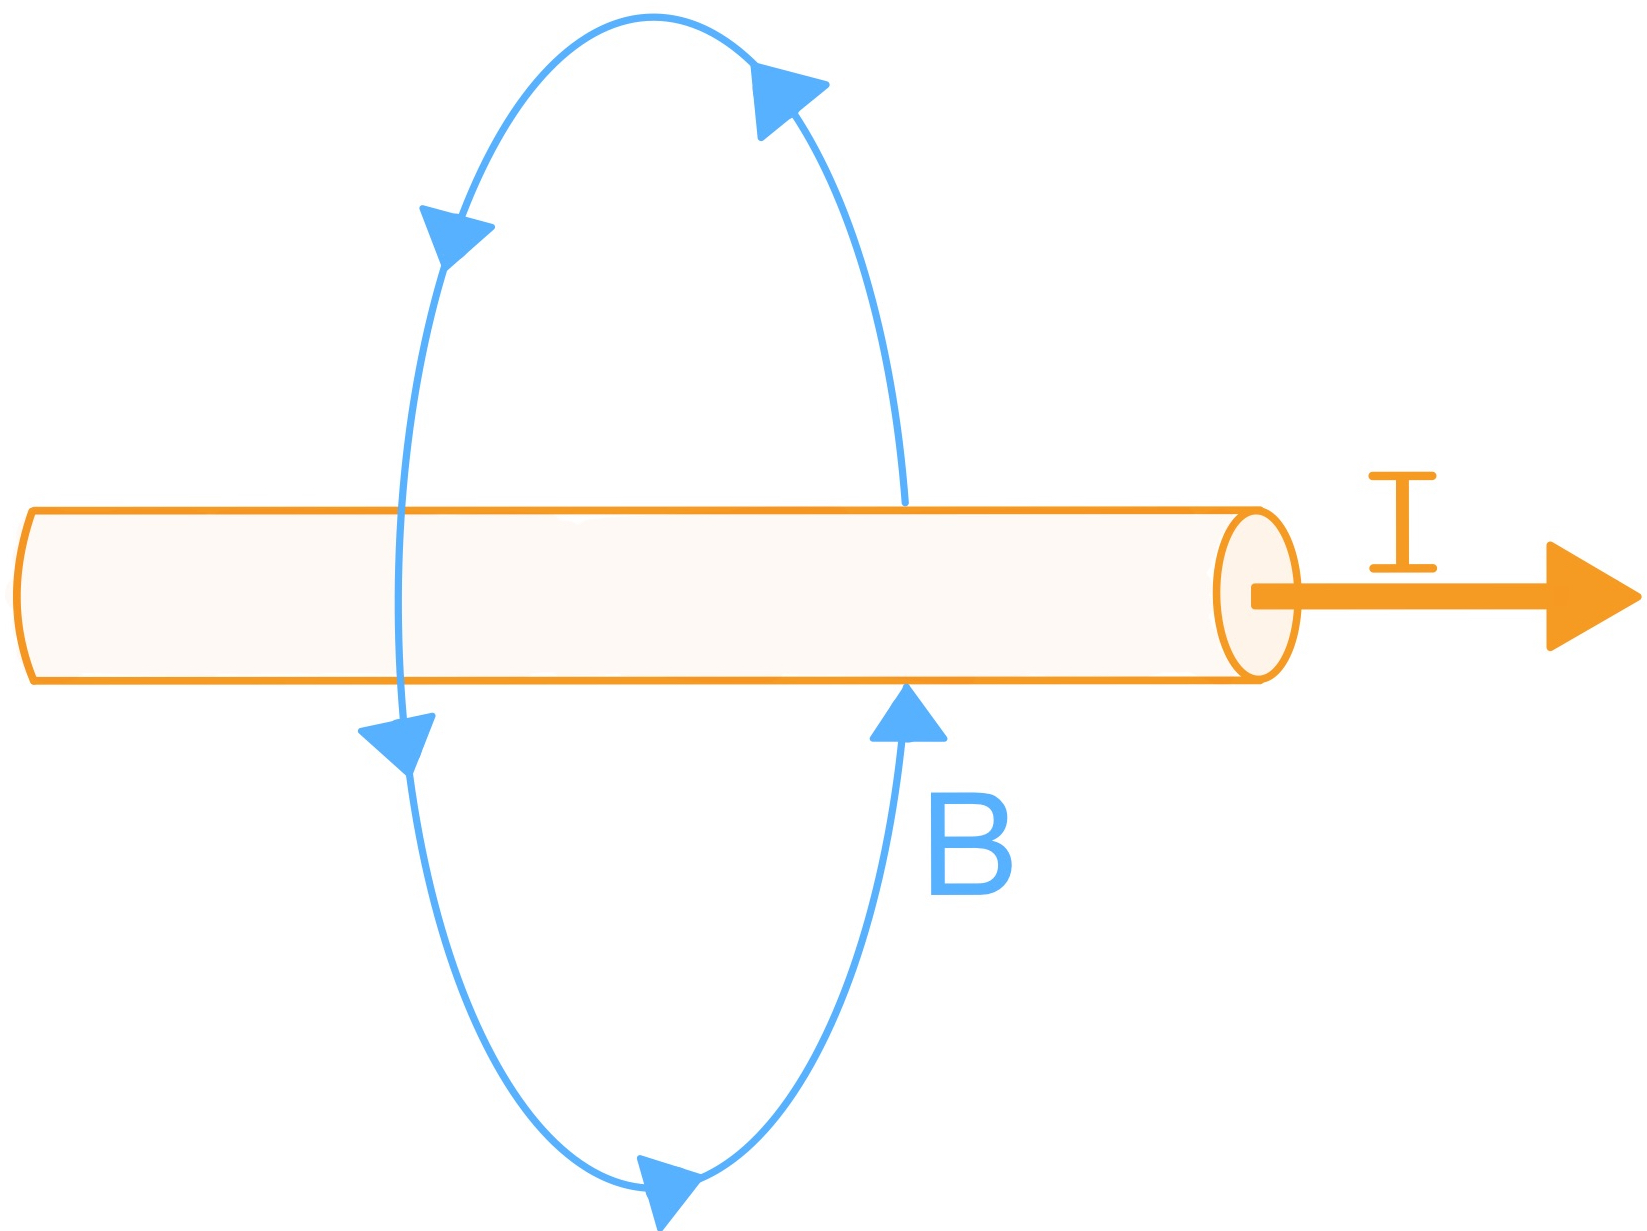
\includegraphics[width=7cm]{FigurasMemoria/amperelaw.jpg}
    \caption{Visualización del campo magnético de un conductor. Elaboración propia.}
    \label{fig:amperelaw} %Para referenciar -> \ref{fig:figNum}
\end{figure}

Una vez entendido el comportamiento en un conductor, el siguiente paso es analizar el componente principal de la lanzadera: la \textbf{bobina}. Una bobina, o solenoide, es un conductor enrollado de manera cilíndrica alrededor de un núcleo de algún material. El número de vueltas que da el conductor alrededor del núcleo se define como espiras y se denota como \textit{N}, y el núcleo posee un parámetro físico llamado permeabilidad relativa \textit{\(\mu_r\)}, que indica su capacidad para permitir el paso del flujo magnético. El siguiente paso por tanto es llegar a una expresión para el campo magnético alrededor de un solenoide. Para ello, partiremos de la ley integral de Ampère y consideraremos un solenoide con \textit{N} espiras y longitud \textit{L}, por el cual pasa una corriente \textit{I}. Elegimos una trayectoria rectangular C que va parcialmente dentro y fuera del solenoide, la cual es conveniente porque simplifica los cálculos del campo magnético.

\begin{figure}[H]
    \centering %\raggedleft \raggedright
    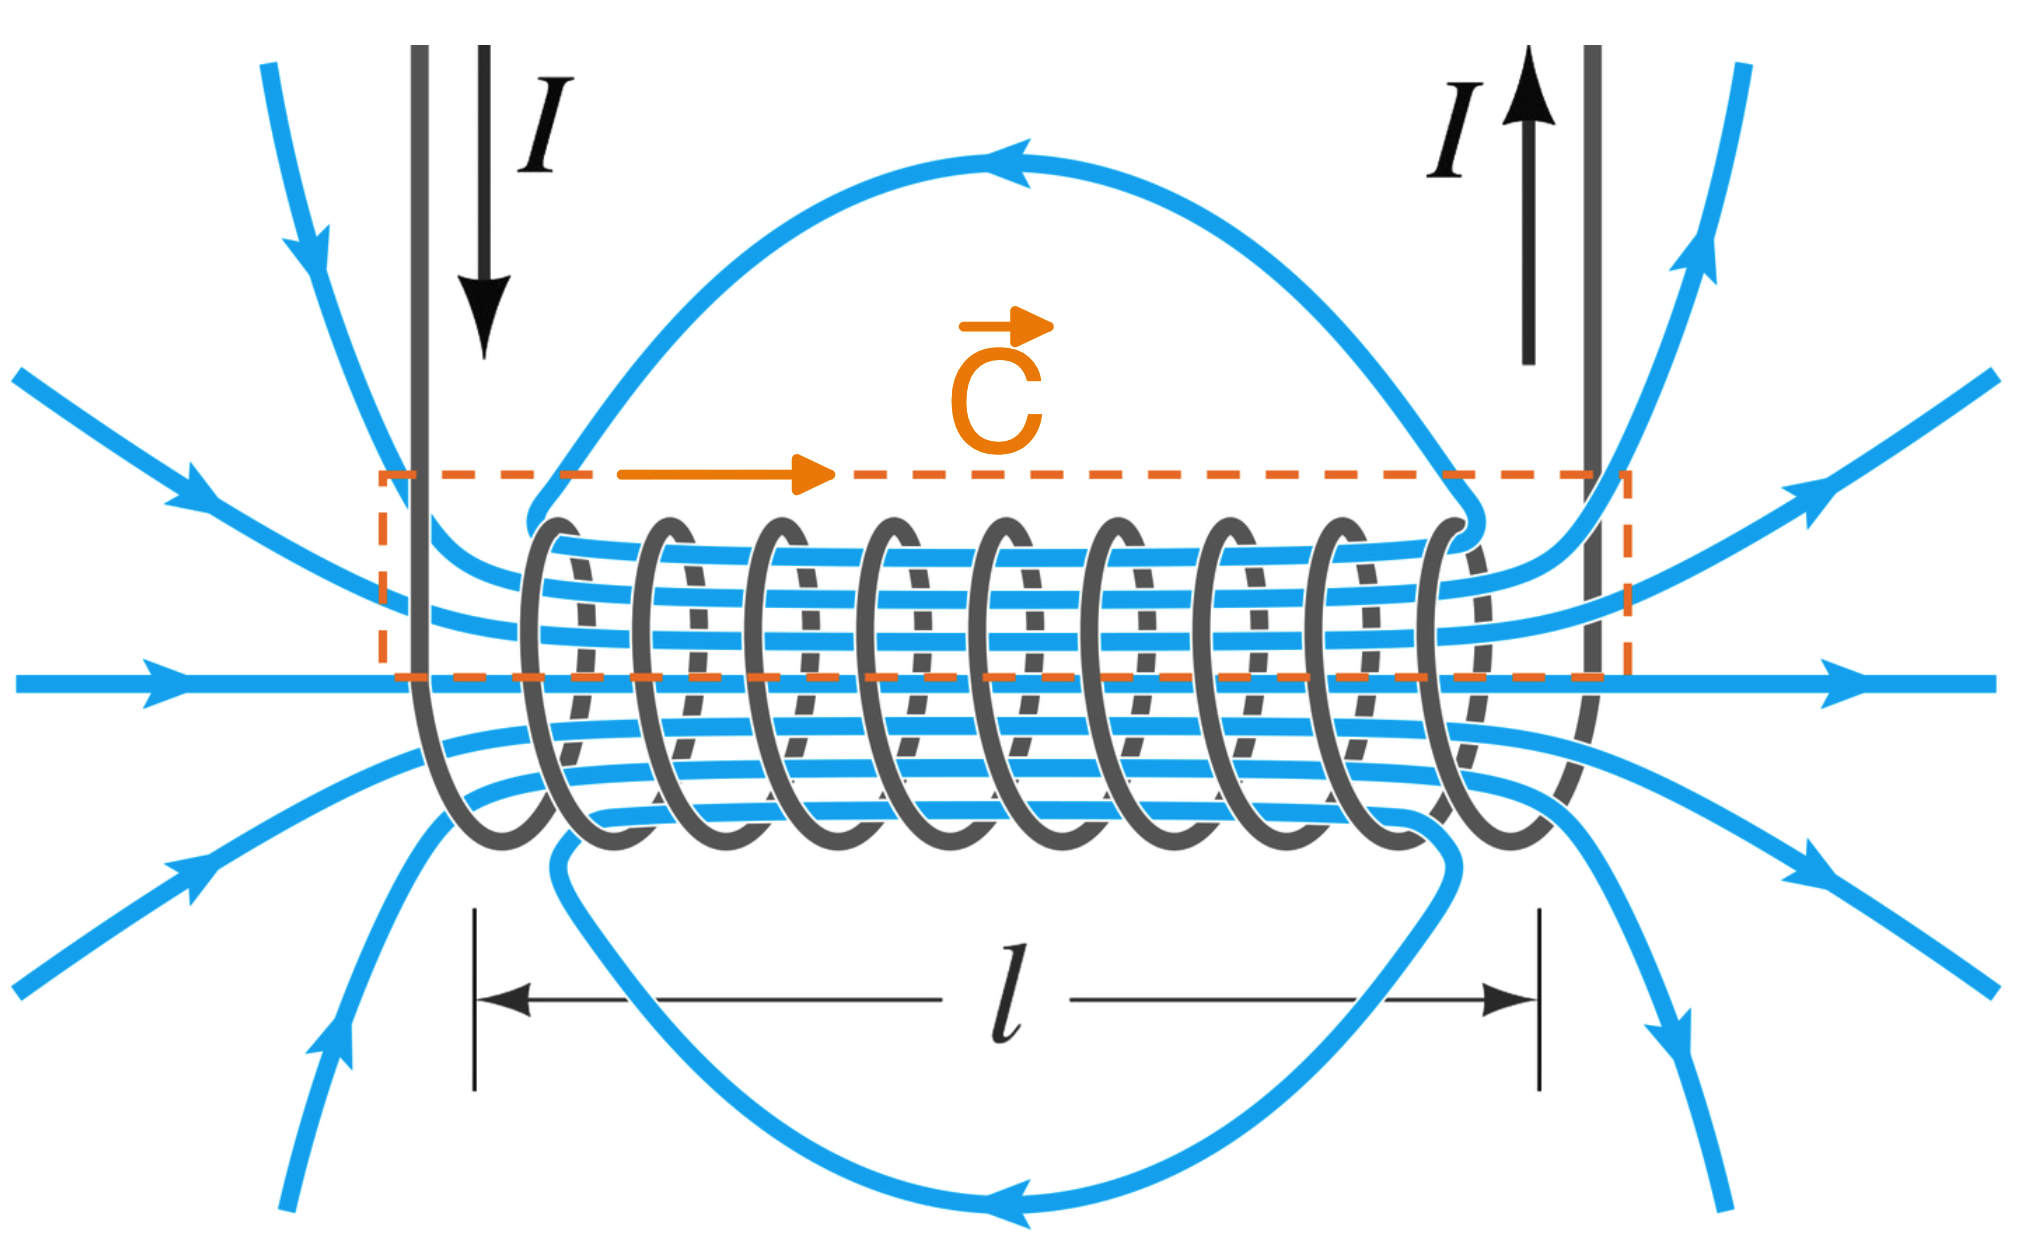
\includegraphics[width=9cm]{FigurasMemoria/integralampere.png}
    \caption{Curva \textbf{C} para la cual realizaremos los cálculos.Imagen tomada de \href{URL}{https://artpictures.club/autumn-2023.html}.}
    \label{fig:integralampere} %Para referenciar -> \ref{fig:figNum}
\end{figure}

La integral de línea del campo magnético \textit{B} en la trayectoria rectangular \(\vec C\) se puede dividir en cuatro segmentos:
\begin{itemize}
    \item Dentro del solenoide, paralelo al eje del solenoide, longitud \textit{l}.
    \item Fuera del solenoide, paralelo al eje del solenoide, longitud \textit{l}.
    \item Dos segmentos perpendiculares al eje del solenoide, cada uno de longitud \textit{w}.
\end{itemize}

Debido a la simetría y a que el solenoide es muy largo, asumimos que el campo magnético fuera del solenoide es despreciable, y el campo dentro es uniforme y paralelo al eje del solenoide. Así, la integral se simplifica a:

\begin{center}
    \[\oint_c\vec{B} \vec{dl}=Bl\]
\end{center}

Analizaremos ahora la corriente encerrada total, que será igual a la corriente que fluye por las \textit{N} espiras:

\begin{center}
    \[I_{encerrada} = NI\]
\end{center}

En una longitud cualquiera, \textit{L}, podemos hablar de una densidad de espiras igual a \(n=\frac{N}{L}\), por lo que en la curva \textit{C} tendremos:

\begin{center}
    \[I_{encerrada} = nIl\]
\end{center}

Ya tenemos los dos términos de la ecuación integral de Ampère, por lo que podemos igualar:

\begin{center}
    \[Bl=\mu_0nIl\to B=\mu_0nI~~\forall n=\frac{N}{L}\to B=\mu_0\frac{NI}{L}\]
\end{center}

Que es la expresión para la inducción electromagnética en un solenoide.

El siguiente punto de interés, con el cual además terminaré el marco teórico, es la forma del campo magnético del solenoide. La geometría del mismo juega un papel crucial en la distribución del campo magnético. Debido a su forma cilíndrica y a la disposición de las espiras, el campo magnético generado en el interior del solenoide es casi uniforme y paralelo al eje del cilindro, variando solo en los extremos donde se curva hacia el núcleo para cumplir la ley de Gauss para el campo magnético (\(\nabla B=0\)). Esta uniformidad del campo magnético es una característica deseable en muchas aplicaciones, como en el diseño de inductores o transformadores. En nuestro caso, la uniformidad del campo nos va a permitir acelerar el proyectil de la lanzadera de manera rectilínea hacia el centro de la bobina.\citep{purcell2013electricidad} \citep{griffiths2005}\citep{tipler2008}.

\begin{figure}[H]
    \centering %\raggedleft \raggedright
    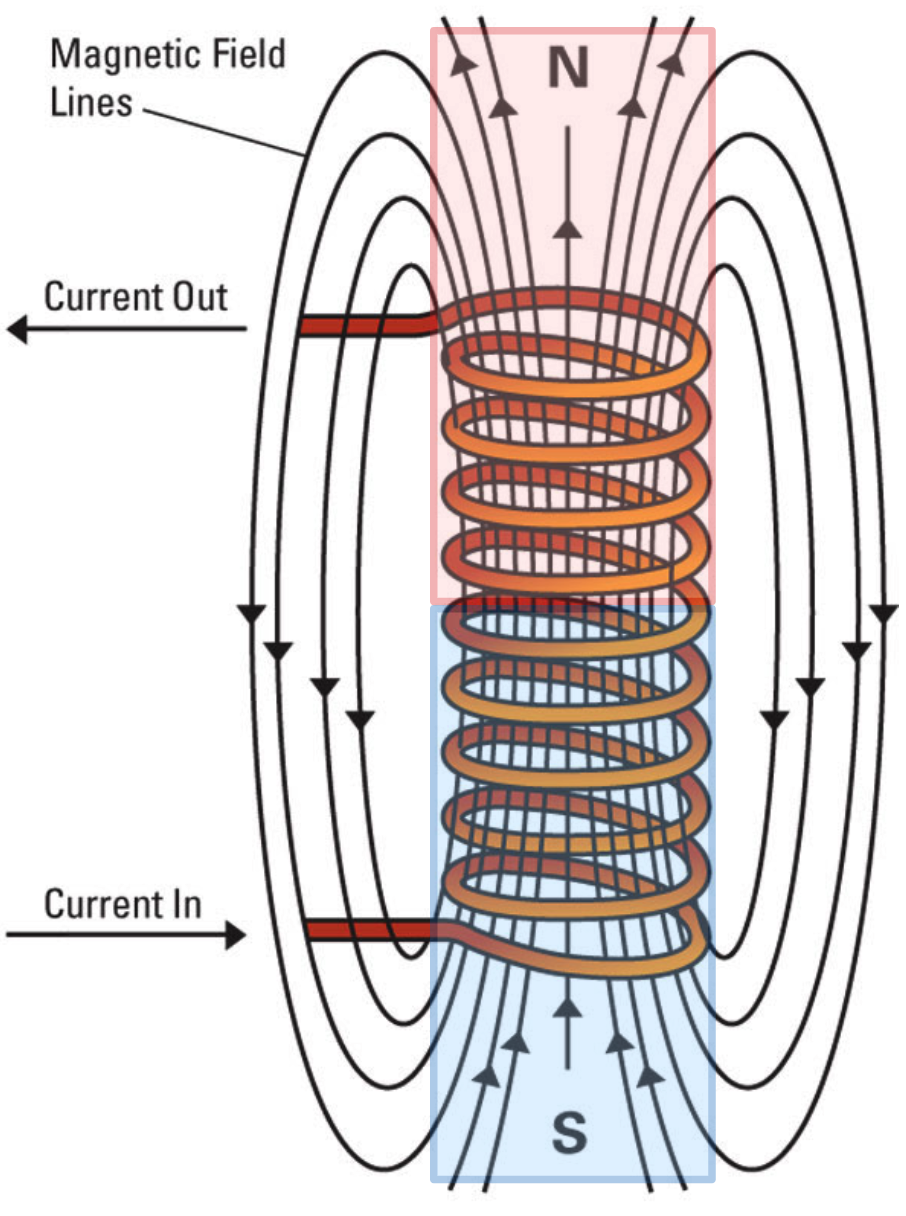
\includegraphics[width=6.5cm]{FigurasMemoria/electromagnet.png}
    \caption{Visualización del campo magnético de una bobina energizada. Imagen tomada de \href{URL}{https://ece.northeastern.edu/fac-ece/nian/mom/electromagnets.html}.}
    \label{fig:electromagnet} %Para referenciar -> \ref{fig:figNum}
\end{figure}

La forma en que aprovecharé este fenómeno para construir la lanzadera consiste en colocar un proyectil de material ferromagnético en el extremo de una bobina energizada, el cual será atraído hacia el centro debido al campo magnético. Justo cuando los centros del proyectil y la bobina coincidan, la corriente se interrumpirá, evitando que el proyectil siga siendo atraído por el electroimán y permitiéndole avanzar por inercia. Esto se logrará mediante un circuito electrónico que energizará la bobina durante el tiempo necesario para que el proyectil alcance la máxima velocidad posible. Este circuito será desarrollado en la sección de prototipo (\ref{subsec:prototipo}).

Para finalizar el marco teórico, presentaré un esquema básico de montaje que servirá como preámbulo al desarrollo de las siguientes partes:

\begin{figure}[H]
    \centering %\raggedleft \raggedright
    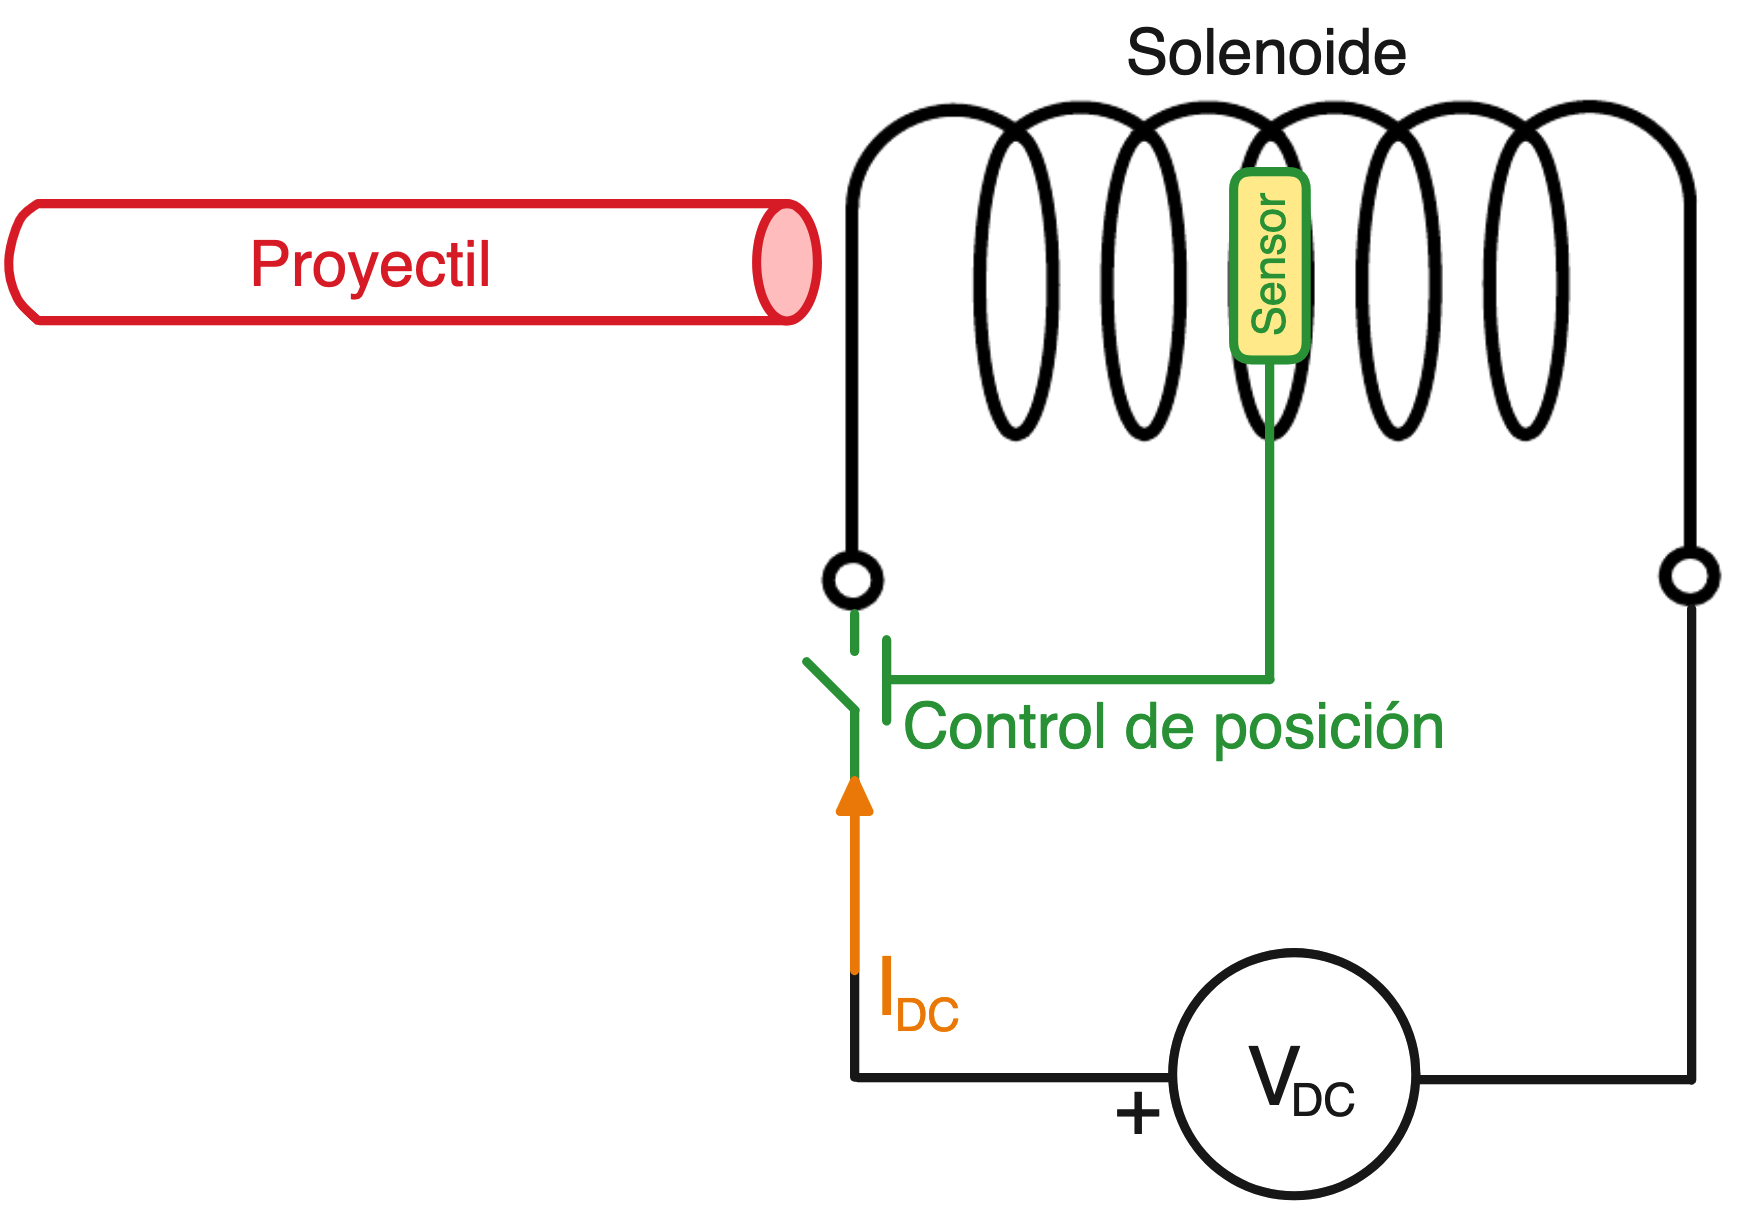
\includegraphics[width=13cm]{FigurasMemoria/esquemabasico.png}
    \caption{Esquema cualitativo de la lanzadera electromagnética. Elaboración propia.}
    \label{fig:esquemabasico} %Para referenciar -> \ref{fig:figNum}
\end{figure}
